
We derived the linear relation between the CR and SRs in each channel 
by fitting a linear function to the ratios of the normalized 
CR and SR sideband background shapes.  This appendix tests the validity of this relationship 
inside the blinded Higgs mass window and determines the potential bias that of the linear transfer function assumption. 

We perform the test by first independently fitting the Bernstein O3 function
 to the sidebands of SR and CR of the \twocentral regions and obtain 
two functions, $f_{bkg}(SR)$ and $f_{bkg}(CR)$. An Asimov dataset 
is generated by $f_{bkg}(SR)$ with $\mu_{inj}=1$. Then we fit this 
Asimov dataset with $f_{bkg}(CR)$ multiplied by a linear function and a floating 
signal contribution, while the parameters of $f_{bkg}(CR)$ are fixed. The test 
 compares the background shapes of SR and CR and measures the difference 
in terms of signal size when the CR background is allowed to vary by a linear 
function. The test for the three signal regions of \twocentral channel is shown in 
Fig. \ref{fig:LinearTest}. We observe, for instance, that even the sidebands of CR and SRIII 
are compatible with a linear transfer function as shown in Sec. \ref{sec:fitbkgds}, 
the background shapes could still differ significantly inside the Higgs mass window which 
could not be covered by linear degrees of freedom. 


\begin{figure}[htbp]
  \centering
 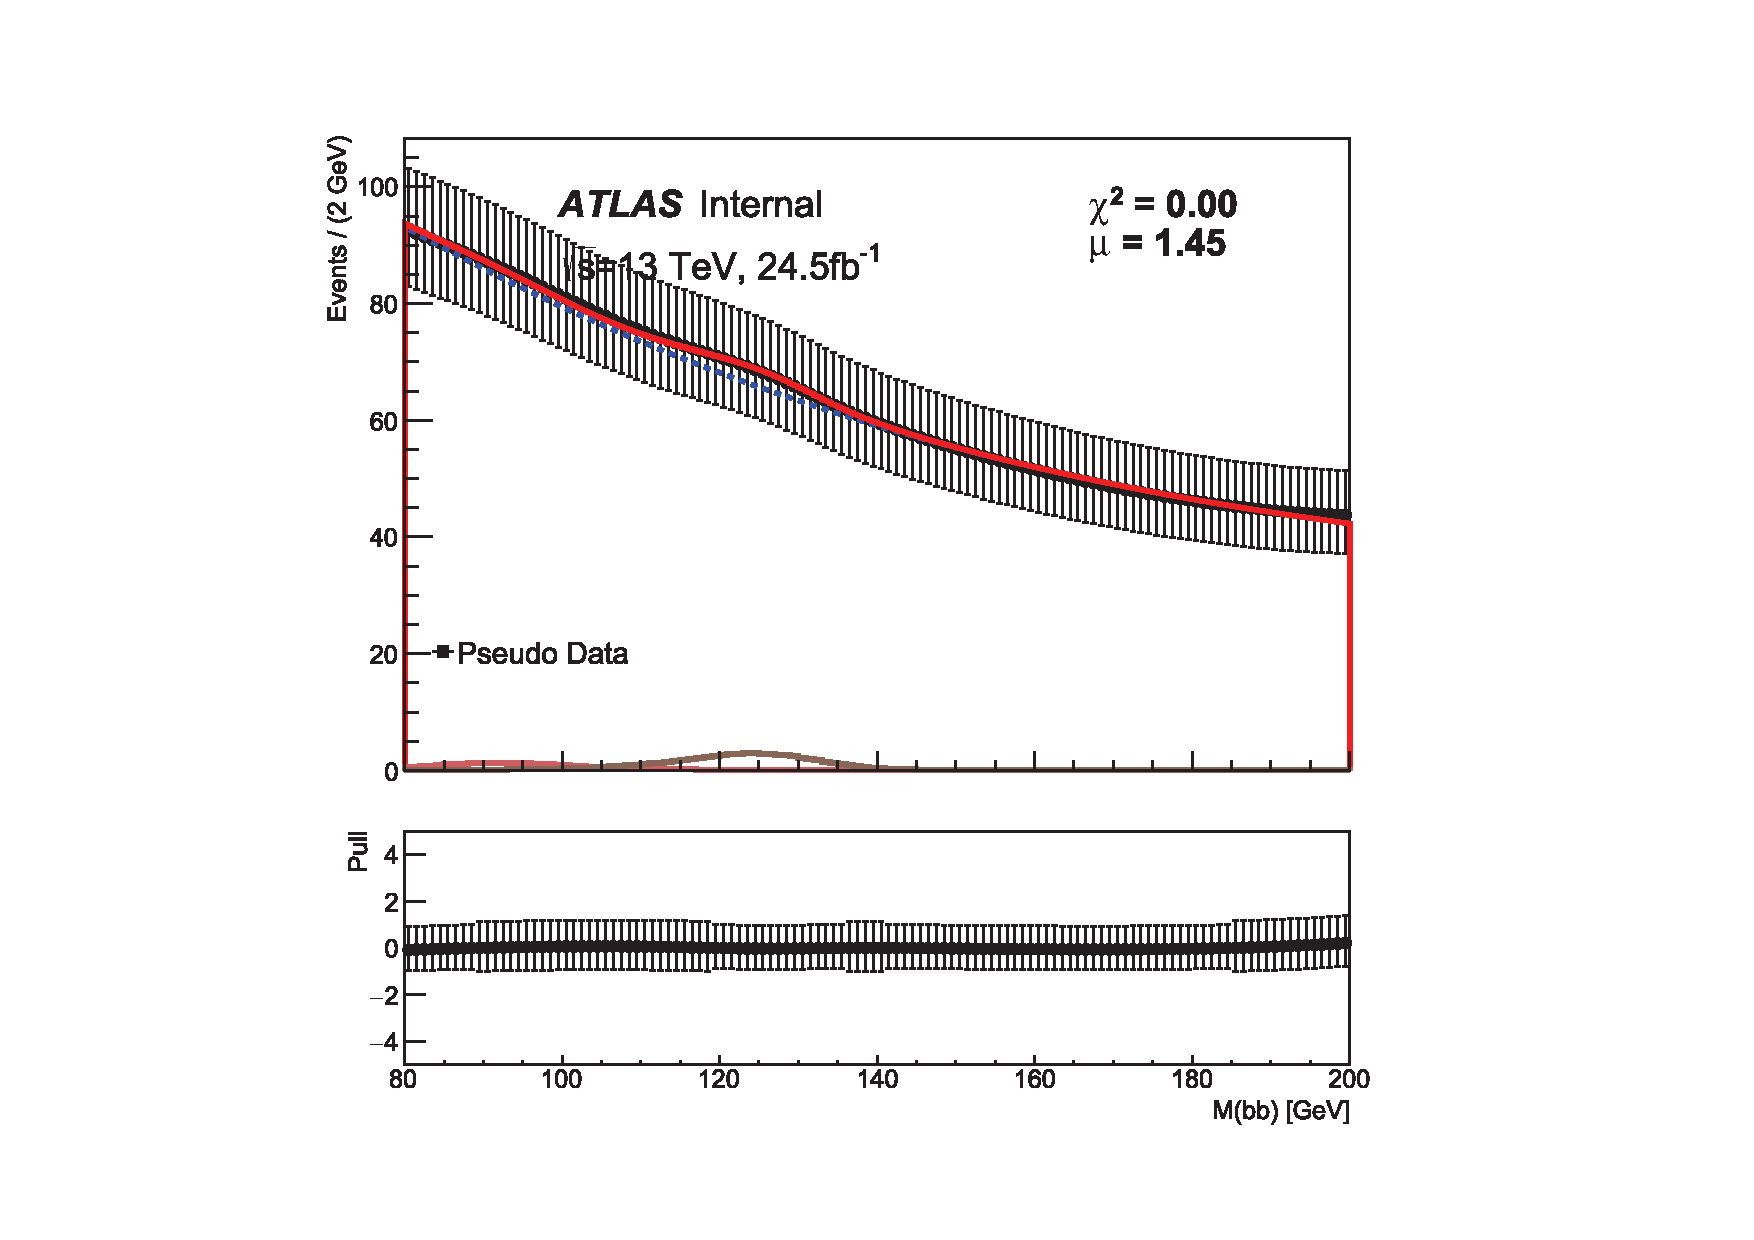
\includegraphics[width=0.49\textwidth]{figures/LinearityTest/LinTest_2cen_SRI.pdf}
 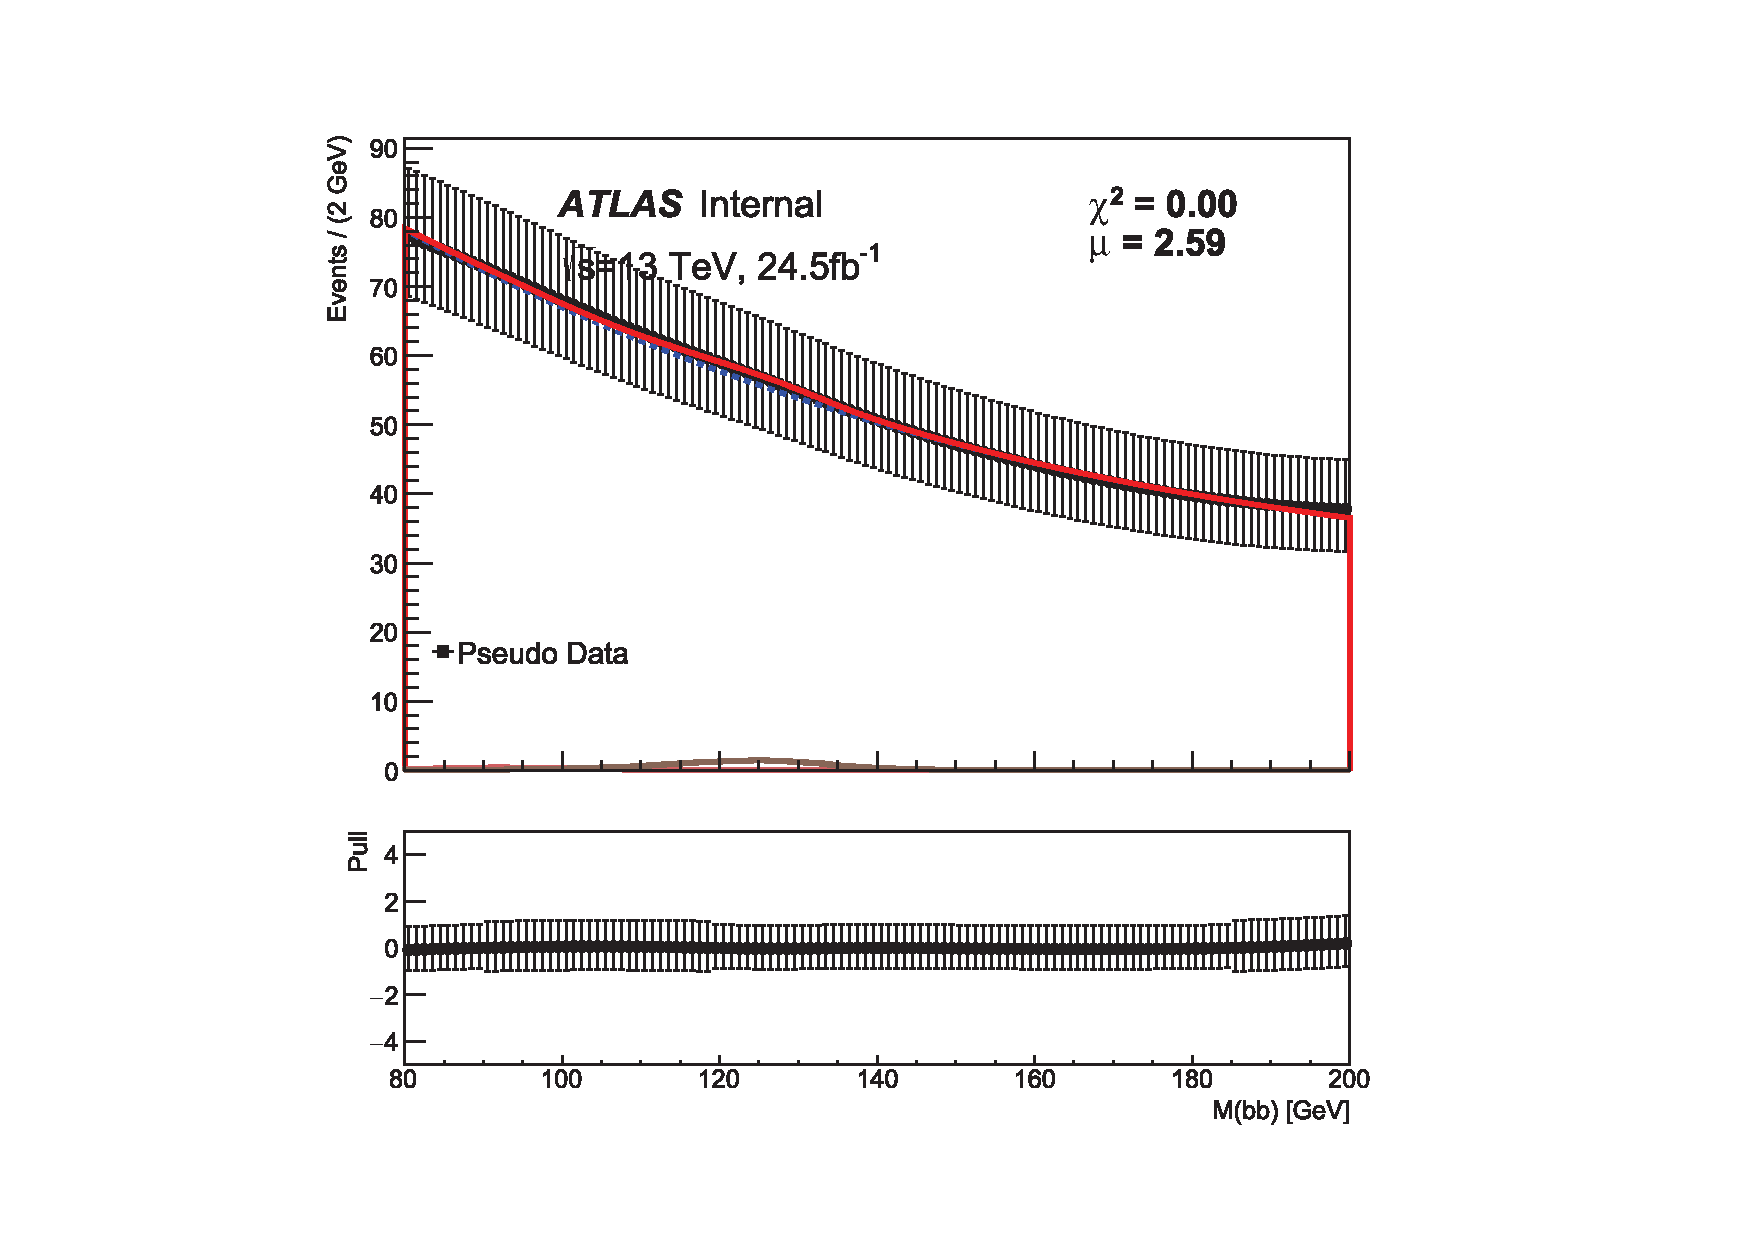
\includegraphics[width=0.49\textwidth]{figures/LinearityTest/LinTest_2cen_SRII.pdf}\\
 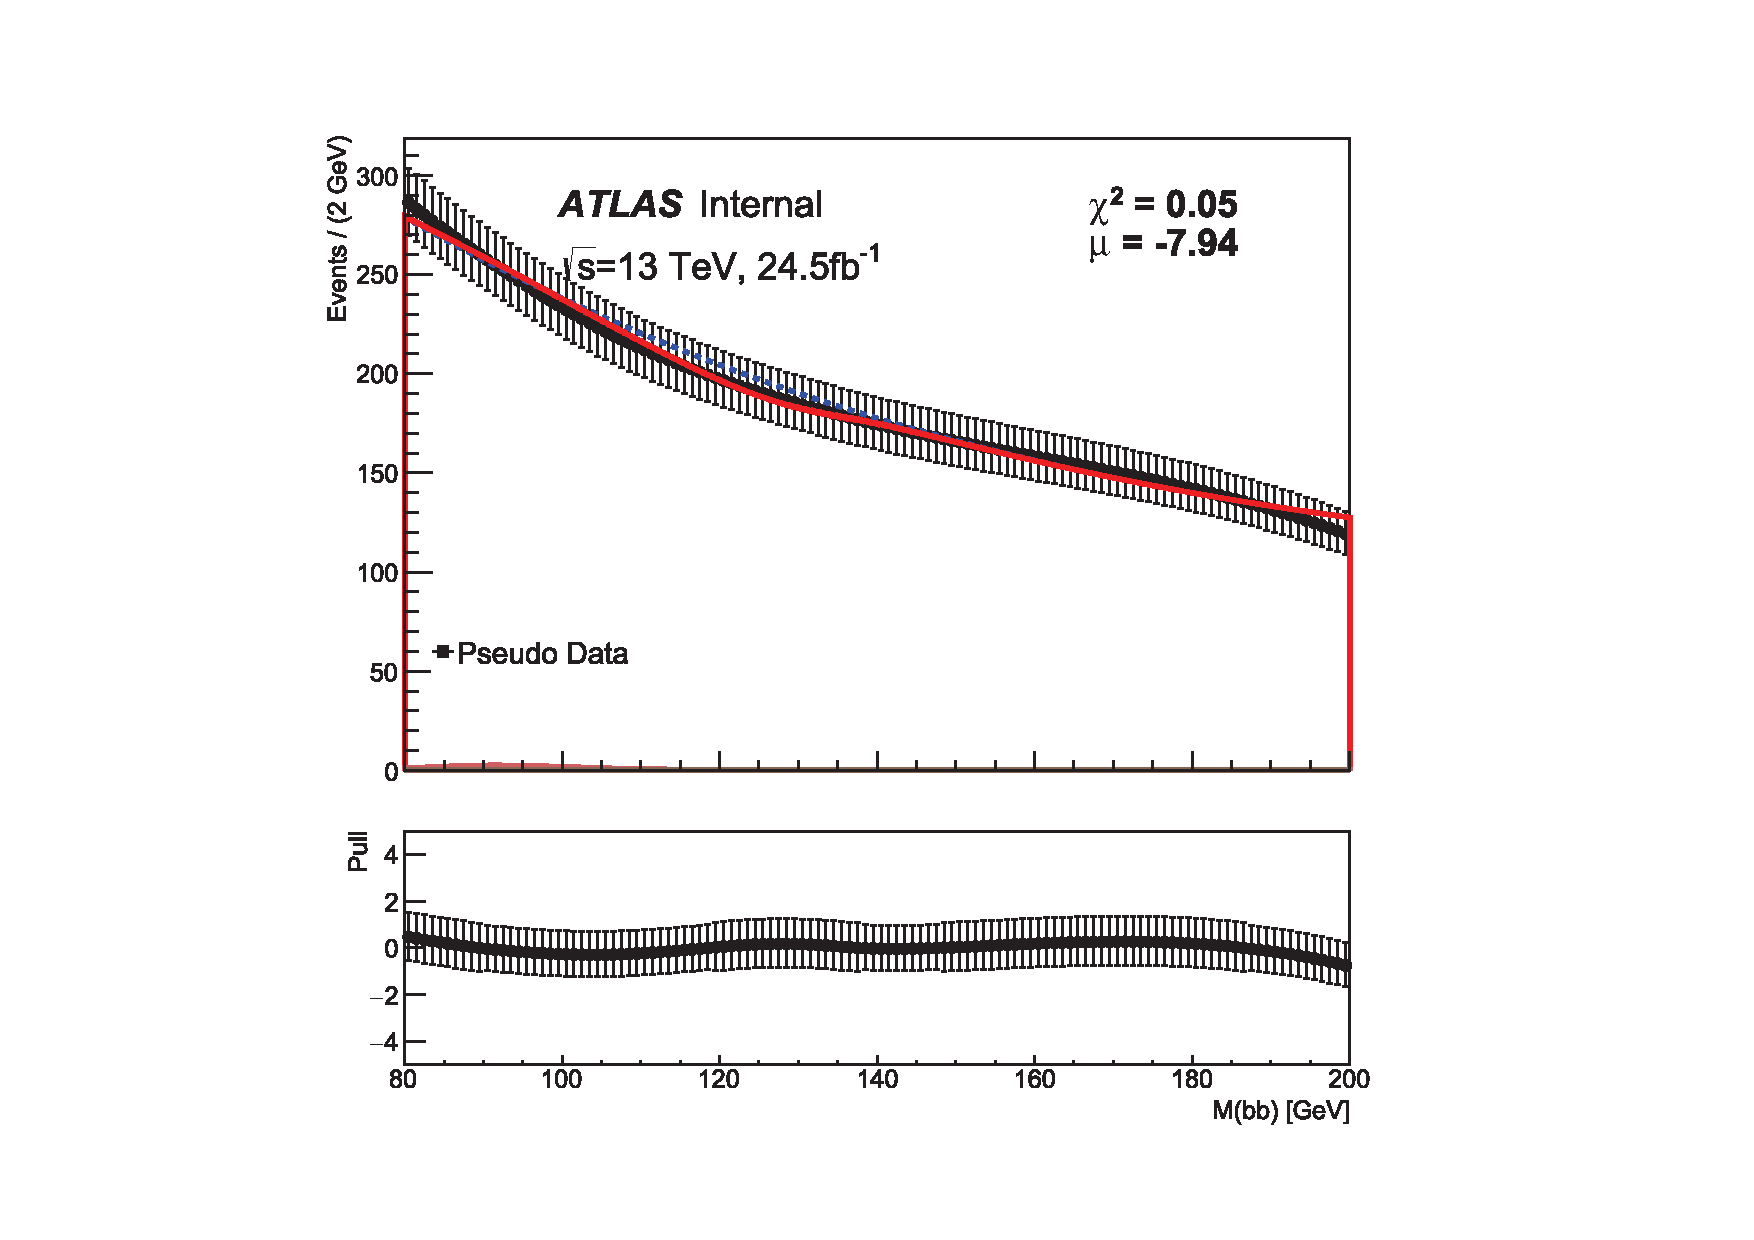
\includegraphics[width=0.49\textwidth]{figures/LinearityTest/LinTest_2cen_SRIII.pdf}\\

\caption{Test of background similarity assumption for \twocentral SRI (top left), SRII (top right) and SRIII (bottom).
The bias of $\mu_{H}$ for each region if the SRs adopt the same background shape as CR multiplied by a linear function 
could be 40\%, and 159\% and 894\%. }
  \label{fig:LinearTest}
\end{figure}
